% ====================================================================
%  徐森林、薛春华《数学分析》（第一册）
%  \S2.1  函数极限的概念
%  源：原书印刷页 81-99（PDF 物理页 87-105）
% ====================================================================
\section{函数极限的概念}\label{sec:2.1}

温故而知新, 先复习一下映射和函数的概念.

\begin{definition}\label{def:2.1.1}
设 $X, Y$ 为非空集合, 如果对 $\forall x \in X$, 有惟一的 $y \in Y$ 与之对应, 表示为 $y = f(x)$, 其中 $x$ 称为自变量或原像点, $y$ 称为因变量或像点, $f$ 称为(单值)映射或对应规律, 记作
\[
f\colon X\to Y,\quad x\mapsto y = f(x).
\]
$X$ 称为 $f$ 的\textbf{定义域},
\[
f(X)=\{f(x)\mid x\in X\}
\]
称为 $f$ 的\textbf{值域},
\[
f(A)=\{f(x)\mid x\in A\subset X\}\subset Y
\]
称为 $A$ 在 $f$ 下的\textbf{像}.
\[
f^{-1}(B)=\{x\in X\mid f(x)\in B\}\subset X
\]
为 $B$ 在 $f$ 下的\textbf{原像}.
\end{definition}

$f$ 的表示法有下面几种.

(1) \textbf{解析式法}: 如 $y=x^{2}$, $y=e^{x}$, $y=\sin x$.

(2) \textbf{列表法}: $y=f(x)=x^{2}$ 图表为
\begin{center}
\begin{tabular}{c|ccccc}
\hline
$x$ & $1$ & $2$ & $3$ & $\cdots$ \\
\hline
$y$ & $1$ & $4$ & $9$ & $\cdots$ \\
\hline
\end{tabular}
\end{center}

(3) \textbf{图像法}: $y = f(x) = x^{2}$ 的图像为抛物线. 画图先列表、描点再连成曲线(如图~\ref{fig:2.1.1} 所示).

\begin{figure}[htbp]
\centering
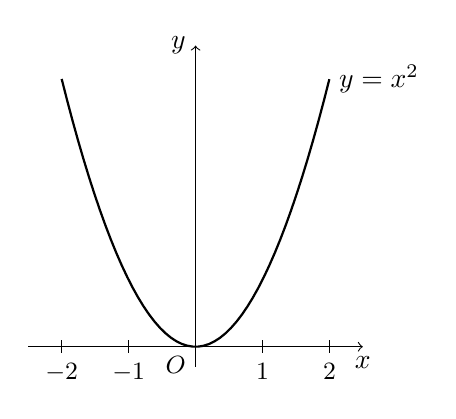
\begin{tikzpicture}[scale=0.85]
  \draw[->] (-2.5,0) -- (2.5,0) node[below] {$x$};
  \draw[->] (0,-0.3) -- (0,4.5) node[left] {$y$};
  \draw[thick, domain=-2:2, samples=50] plot (\x, {\x*\x});
  \node[right] at (2,4) {$y=x^2$};
  \foreach \x in {-2,-1,1,2} {
    \draw (\x,0.1) -- (\x,-0.1) node[below] {\small $\x$};
  }
  \node[below left] at (0,0) {\small $O$};
\end{tikzpicture}
\caption{}\label{fig:2.1.1}
\end{figure}

如果 $\forall x_{1}, x_{2} \in X, x_{1} \neq x_{2}$, 必有 $f(x_{1}) \neq f(x_{2})$, 即若 $f(x_{1})=f(x_{2})$, 必有 $x_{1}=x_{2}$, 则称 $f$ 为\textbf{单射}; 如果 $\forall y\in Y$, 必 $\exists x\in X$, s.t. $f(x)=y$, 则称 $f$ 为\textbf{满射}.

如果 $f$ 既为单射又为满射, 则称 $f$ 为\textbf{双射}或\textbf{一一映射}. 此时, $f$ 有逆映射 $f^{-1}\colon Y \to X$, $x = f^{-1}(y)$ (即 $y = f(x)$). 显然, 当 $f$ 为单射时, $f\colon X \to f(X)$ 就为双射或一一映射.

设 $X$ 为非空集合, $f\colon X \to \mathbb{R}$, $x \mapsto y = f(x)$ 为映射, 则称 $f$ 为\textbf{实(值)函数}, 本书中简称为\textbf{函数}.
\begin{itemize}
  \item 若 $X \subset \mathbb{R}$, 则称 $f$ 为一元(单变量)函数;
  \item 若 $X \subset \mathbb{R}^{2} = \{(x, y) \mid x, y \in \mathbb{R}\}$, 则称 $f$ 为二元函数;
  \item 若 $X \subset \mathbb{R}^{3} = \{(x, y, z) \mid x, y, z \in \mathbb{R}\}$, 则称 $f$ 为三元函数;
  \item 若 $X \subset \mathbb{R}^{n} = \{(x_{1}, x_{2}, \cdots, x_{n}) \mid x_{i} \in \mathbb{R}, i=1,2,\cdots,n\}$, 则称 $f$ 为 $n$ 元函数.
\end{itemize}

设 $f, g\colon X \to \mathbb{R}$, $x \in X$, 令
\begin{align*}
(f\pm g)(x) &= f(x)\pm g(x), \\
(fg)(x) &= f(x)g(x), \\
\frac{f}{g}(x) &= \frac{f(x)}{g(x)}\quad (g(x)\neq 0).
\end{align*}
它们分别定义了 $f$ 与 $g$ 的和函数 $f + g$, 差函数 $f - g$, 积函数 $fg$ 及商函数 $\frac{f}{g}$.

设 $f\colon X \to Y$, $g\colon Y \to Z$, 则称 $g \circ f\colon X \to Z$, $x \mapsto z = g \circ f(x) = g(f(x))$ 为 $f$ 与 $g$ 的复合. 两个函数 $f, g$ 的复合称为 $f$ 与 $g$ 的复合函数(如图~\ref{fig:2.1.2} 所示). 关于复合显然有 $(g \circ f) \circ h = g \circ (f \circ h)$.

\begin{figure}[htbp]
\centering
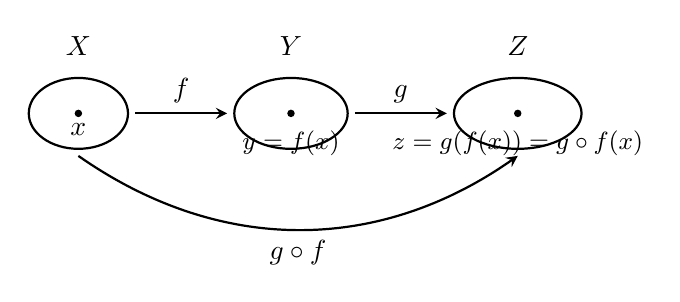
\begin{tikzpicture}[scale=0.9, >=stealth]
  \draw[thick] (0,0) ellipse (0.7cm and 0.5cm) node[above=0.6cm] {$X$};
  \fill (0,0) circle (1.5pt) node[below] {$x$};
  
  \draw[thick] (3.0,0) ellipse (0.8cm and 0.5cm) node[above=0.6cm] {$Y$};
  \fill (3.0,0) circle (1.5pt) node[below=0.1cm] {\small $y=f(x)$};
  
  \draw[thick] (6.2,0) ellipse (0.9cm and 0.5cm) node[above=0.6cm] {$Z$};
  \fill (6.2,0) circle (1.5pt) node[below=0.1cm] {\small $z=g(f(x))=g\circ f(x)$};
  
  \draw[->, thick] (0.8,0) -- (2.1,0) node[midway, above] {$f$};
  \draw[->, thick] (3.9,0) -- (5.2,0) node[midway, above] {$g$};
  \draw[->, thick] (0,-0.6) to[out=-35,in=-145] node[midway, below] {$g\circ f$} (6.2,-0.6);
\end{tikzpicture}
\caption{}\label{fig:2.1.2}
\end{figure}

中学里已学的基本初等函数共有 6 类:

(1) \textbf{常值函数} $y=f(x)=c$, 定义域为 $\mathbb{R}$.

(2) \textbf{幂函数} $y = f(x) = x^{\alpha}$ ($\alpha$ 为实数). 当 $x > 0$ 时, 任何 $\alpha$ 都有意义; $x^{n}\ (n \in \mathbb{N})$ 的定义域为实数集 $\mathbb{R}$; $x^{-n}\ (n \in \mathbb{N})$ 的定义域为 $\mathbb{R} \setminus \{0\}$; $x^{\frac{1}{2}} = \sqrt{x}$ 的定义域为 $[0, +\infty)$; $x^{-\frac{1}{2}}$ 的定义域为 $(0, +\infty)$; $x^{\frac{1}{3}}$ 的定义域为 $\mathbb{R}$; $x^{-\frac{1}{3}}$ 的定义域为 $\mathbb{R} \setminus \{0\}$; 等等.

(3) \textbf{三角函数} $y=\sin x, \cos x$ 定义域都为 $\mathbb{R}$; $y=\tan x$, 定义域为 $\mathbb{R} \setminus \{k\pi + \frac{\pi}{2}, k \in \mathbb{Z}\}$; $y=\cot x$, 定义域为 $\mathbb{R} \setminus \{k\pi, k \in \mathbb{Z}\}$; $y=\sec x$, 定义域为 $\mathbb{R} \setminus \{k\pi + \frac{\pi}{2}, k \in \mathbb{Z}\}$; $y=\csc x$, 定义域为 $\mathbb{R} \setminus \{k\pi, k \in \mathbb{Z}\}$.

(4) \textbf{反三角函数} $y=\arcsin x, \arccos x$ 定义域为 $[-1,1]$; $y=\arctan x, \operatorname{arccot} x$ 定义域为 $\mathbb{R}$.

(5) \textbf{指数函数} $y=a^{x}\ (a>0,a\neq1)$, 定义域为 $\mathbb{R}$.

(6) \textbf{对数函数} $y=\log_{a}x\ (a>0,a\neq1)$, 定义域为 $(0,+\infty)$. 特别地, 常用对数记作 $\lg x = \log_{10}x$, 自然对数记作 $\ln x = \log_{\mathrm{e}}x$.

读者应记住每个基本初等函数的值域, 并画出相应的图形.

\begin{definition}\label{def:2.1.2}
由基本初等函数通过有限次 $+$, $-$, $\cdot$, $\div$ 和复合得到的函数称为\textbf{初等函数}. 这是一类重要的函数.
\end{definition}

再给出几类今后要常用的函数.

\begin{example}\label{ex:2.1.1}
证明:
\begin{enumerate}[label=(\arabic*)]
  \item 双曲函数:
  \begin{align*}
  \sinh x &= \frac{e^{x}-e^{-x}}{2},\quad \cosh x=\frac{e^{x}+e^{-x}}{2}, \\
  \tanh x &= \frac{\sinh x}{\cosh x}=\frac{e^{x}-e^{-x}}{e^{x}+e^{-x}},\quad \coth x=\frac{\cosh x}{\sinh x}=\frac{e^{x}+e^{-x}}{e^{x}-e^{-x}}
\end{align*}
  都是初等函数. 读者经过验算可知双曲函数具有性质:
  \[
  \sinh 2x=2\sinh x\cosh x,\quad \cosh 2x=\cosh^{2}x+\sinh^{2}x,\quad \cosh^{2}x-\sinh^{2}x=1.
\]
  \item $y=\ln(x+\sqrt{x^{2}+1})$ 为初等函数.
  \item $y=|x|=\begin{cases} x, & x\geqslant0, \\ -x, & x<0 \end{cases}$ 为初等函数.
  \item 多项式函数 $y = a_{0}x^{n} + a_{1}x^{n-1} + \cdots + a_{n-1}x + a_{n}\ (a_{0} \neq 0)$ 与有理函数
  \[
  y = \frac{a_{0}x^{n} + a_{1}x^{n-1} + \cdots + a_{n-1}x + a_{n}}{b_{0}x^{m} + b_{1}x^{m-1} + \cdots + b_{m-1}x + b_{m}}\quad (a_{0} \neq 0, b_{0} \neq 0)
\]
  均为初等函数.
\end{enumerate}
\end{example}

\begin{proof}
(1) 以 $y = \tanh x$ 为例证明双曲函数为初等函数. 因为 $y = \tanh x = \frac{e^{x} - e^{-x}}{e^{x} + e^{-x}}$ 为基本初等函数 $e^{x}, e^{-x} = (e^{-1})^{x}$ 通过一次减法、一次加法、一次除法得到, 所以它为初等函数. 或者因为 $y = \tanh x = \frac{e^{x} - \frac{1}{e^{x}}}{e^{x} + \frac{1}{e^{x}}}$ 为基本初等函数 $e^{x}, 1$ 通过一次减法, 一次加法, 三次除法得到, 所以它为初等函数. 其他类似证明.

(2) 因为 $y=\ln(x+\sqrt{x^{2}+1})$ 由基本初等函数 $x, x^{2}, 1, \sqrt{x}, \ln x$ 通过两次加法, 两次复合得到, 所以它为初等函数.

(3) 因为 $y=|x|=\sqrt{x^{2}}$ 为基本初等函数 $x^{2}, \sqrt{x}$ 通过一次复合得到, 所以它为初等函数.

(4) 因为多项式函数 $y=a_{0}x^{n}+\cdots+a_{n}$ 为基本初等函数 $a_{0}, \cdots, a_{n}, x, \cdots, x^{n}$ 通过 $n$ 次乘法与 $n$ 次加法得到, 所以它为初等函数.

而有理函数为基本初等函数通过有限次乘法、加法以及除法得到, 所以它为初等函数.
\end{proof}

\begin{example}\label{ex:2.1.2}
\begin{enumerate}[label=(\arabic*)]
  \item 设 $f_{1}, f_{2}, \cdots, f_{n}$ 都为初等函数, 则由 $f_{1}, f_{2}, \cdots, f_{n}$ 经有限次 $+$, $-$, $\cdot$, $\div$, 复合运算得到的函数 $f$ 仍为初等函数.
  \item 设 $f, g$ 都为初等函数, 则 $\max\{f, g\}$ 与 $\min\{f, g\}$ 均为初等函数.
\end{enumerate}
\end{example}

\begin{proof}
(1) 因为 $f_{1}, f_{2}, \cdots, f_{n}$ 都为初等函数, 所以它们都由基本初等函数通过有限次 $+$, $-$, $\cdot$, $\div$, 复合运算得到. 从而, 由 $f_{1}, f_{2}, \cdots, f_{n}$ 经有限次 $+$, $-$, $\cdot$, $\div$, 复合运算得到的函数 $f$ 也由基本初等函数通过有限次 $+$, $-$, $\cdot$, $\div$, 复合运算得到, 该函数 $f$ 应是初等函数.

(2) 由 $f, g$ 都为初等函数及
\begin{align*}
\max\{f,g\} &= \frac{(f+g)+|f-g|}{2}=\frac{(f+g)+\sqrt{(f-g)^2}}{2}, \\
\min\{f,g\} &= \frac{(f+g)-|f-g|}{2}=\frac{(f+g)-\sqrt{(f-g)^2}}{2}
\end{align*}
或 $\min\{f,g\} = -\max\{-f,-g\}$ 可知 $\max\{f,g\}$ 与 $\min\{f,g\}$ 均为初等函数.
\end{proof}

另一类重要的函数就是\textbf{分段函数}, 即每一段上用不同的式子表达的函数.

\begin{example}\label{ex:2.1.3}
\begin{enumerate}[label=(\arabic*)]
  \item \textbf{符号函数}(如图~\ref{fig:2.1.3} 所示):
  \[
  y=\operatorname{sgn} x=\begin{cases}
  1, & x>0, \\
  0, & x=0, \\
  -1, & x<0.
\end{cases}
\]
  \item \textbf{“取整数”函数}(如图~\ref{fig:2.1.4} 所示):
  \[
  y=\lfloor x\rfloor = [x]
\]
  为不大于 $x$ 的最大整数, 此时有 $x-1<[x]\leqslant x<[x]+1$.
\end{enumerate}
\end{example}

\begin{figure}[htbp]
\centering
\begin{minipage}[t]{0.45\textwidth}
\centering
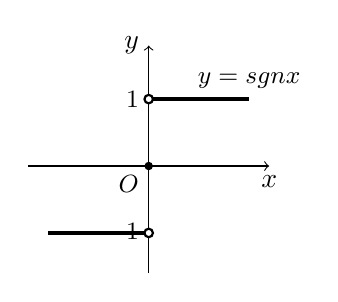
\begin{tikzpicture}[scale=0.85]
  \draw[->] (-1.8,0) -- (1.8,0) node[below] {$x$};
  \draw[->] (0,-1.6) -- (0,1.8) node[left] {$y$};
  \node[below left] at (0,0) {\small $O$};
  \draw[very thick] (0,1) -- (1.5,1) node[above, font=\small] {$y=\operatorname{sgn} x$};
  \draw[very thick] (-1.5,-1) -- (0,-1);
  \filldraw[fill=white, draw=black, thick] (0,1) circle (1.8pt);
  \filldraw[fill=white, draw=black, thick] (0,-1) circle (1.8pt);
  \fill (0,0) circle (1.8pt);
  \node[left] at (0,1) {\small $1$};
  \node[left] at (0,-1) {\small $-1$};
\end{tikzpicture}
\caption{}\label{fig:2.1.3}
\end{minipage}
\hfill
\begin{minipage}[t]{0.45\textwidth}
\centering
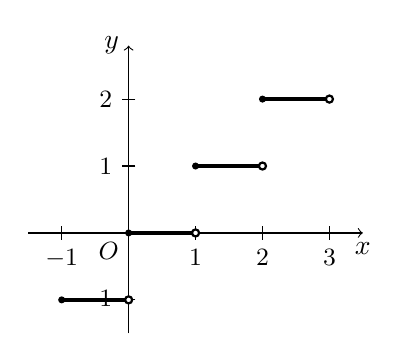
\begin{tikzpicture}[scale=0.85]
  \draw[->] (-1.5,0) -- (3.5,0) node[below] {$x$};
  \draw[->] (0,-1.5) -- (0,2.8) node[left] {$y$};
  \node[below left] at (0,0) {\small $O$};
  \foreach \x in {-1,1,2,3} {
    \draw (\x,0.1) -- (\x,-0.1) node[below] {\small $\x$};
  }
  \foreach \y in {-1,1,2} {
    \draw (0.1,\y) -- (-0.1,\y) node[left] {\small $\y$};
  }
  \draw[very thick] (-1,-1) -- (0,-1);
  \fill (-1,-1) circle (1.5pt);
  \filldraw[fill=white, draw=black, thick] (0,-1) circle (1.5pt);
  
  \draw[very thick] (0,0) -- (1,0);
  \fill (0,0) circle (1.5pt);
  \filldraw[fill=white, draw=black, thick] (1,0) circle (1.5pt);
  
  \draw[very thick] (1,1) -- (2,1);
  \fill (1,1) circle (1.5pt);
  \filldraw[fill=white, draw=black, thick] (2,1) circle (1.5pt);
  
  \draw[very thick] (2,2) -- (3,2);
  \fill (2,2) circle (1.5pt);
  \filldraw[fill=white, draw=black, thick] (3,2) circle (1.5pt);
\end{tikzpicture}
\caption{}\label{fig:2.1.4}
\end{minipage}
\end{figure}

\begin{enumerate}[label=(\arabic*), resume]
  \item \textbf{尾数函数}(如图~\ref{fig:2.1.5} 所示):
  \[
  y=x-[x]\overset{\mathrm{def}}{=}\{x\},
\]
  则 $0\leqslant\{x\}<1$, 且 $\{x\}$ 是以 $1$ 为周期的函数.
  \item \textbf{绝对值函数}(如图~\ref{fig:2.1.6} 所示):
  \[
  y=|x|=\begin{cases}
  x, & x\geqslant0, \\
  -x, & x<0.
\end{cases}
\]
  \item 设 $A \subseteq \mathbb{R}$, $A$ 的\textbf{特征函数} $\chi_{A}\colon \mathbb{R} \to \mathbb{R}$,
  \[
  \chi_{A}(x)=\begin{cases}
  1, & x\in A, \\
  0, & x\in\mathbb{R}\setminus A\ (\text{即 } x\notin A).
\end{cases}
\]
  \item \textbf{Dirichlet 函数}:
  \[
  D(x)=\begin{cases}
  1, & x\in\mathbb{Q}, \\
  0, & x\in\mathbb{R}\setminus\mathbb{Q},
\end{cases}
\]
  它是 $\mathbb{Q}$ 的特征函数.
\end{enumerate}

以上 6 个函数都为分段函数.

\begin{figure}[htbp]
\centering
\begin{minipage}[t]{0.45\textwidth}
\centering
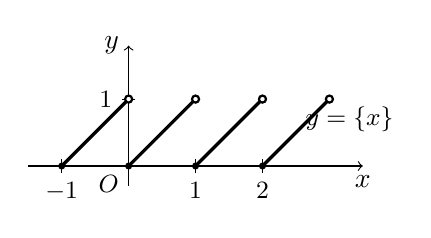
\begin{tikzpicture}[scale=0.85]
  \draw[->] (-1.5,0) -- (3.5,0) node[below] {$x$};
  \draw[->] (0,-0.3) -- (0,1.8) node[left] {$y$};
  \node[below left] at (0,0) {\small $O$};
  \draw (0.1,1) -- (-0.1,1) node[left] {\small $1$};
  \foreach \x in {-1,1,2} {
    \draw (\x,0.1) -- (\x,-0.1) node[below] {\small $\x$};
  }
  \foreach \k in {-1,0,1,2} {
    \draw[very thick] (\k,0) -- (\k+1,1);
    \fill (\k,0) circle (1.5pt);
    \filldraw[fill=white, draw=black, thick] (\k+1,1) circle (1.5pt);
  }
  \node[right, font=\small] at (2.5,0.7) {$y=\{x\}$};
\end{tikzpicture}
\caption{}\label{fig:2.1.5}
\end{minipage}
\hfill
\begin{minipage}[t]{0.45\textwidth}
\centering
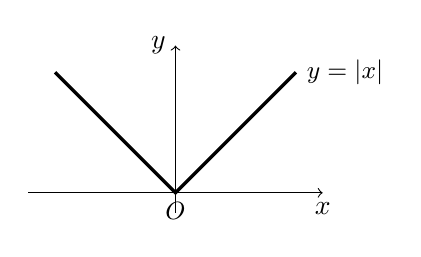
\begin{tikzpicture}[scale=0.85]
  \draw[->] (-2.2,0) -- (2.2,0) node[below] {$x$};
  \draw[->] (0,-0.3) -- (0,2.2) node[left] {$y$};
  \node[below] at (0,0) {\small $O$};
  \draw[very thick] (-1.8,1.8) -- (0,0) -- (1.8,1.8) node[right, font=\small] {$y=|x|$};
\end{tikzpicture}
\caption{}\label{fig:2.1.6}
\end{minipage}
\end{figure}

回想一下数列极限 $\lim\limits_{n\to+\infty}a_n=\lim\limits_{n\to+\infty}f(n)=a\in\mathbb{R}$ (收敛), $+\infty, -\infty, \infty$, 共有 4 种. 用 $N$ 刻画 $n$ 趋于 $+\infty$ 的程度, 用 $\varepsilon>0$ 刻画 $a_n$ 靠近 $a$ 的程度, 用 $A$ 刻画 $a_n$ 趋于 $+\infty, -\infty, \infty$ 的程度. 这里自变量只有一个趋向 $n\to+\infty$, 而一般函数 $f(x)$ 除了 $x\to+\infty$ 外, 还有 $x\to x_0, x_0^+, x_0^-, x\to-\infty, \infty$ 等情况.

我们考虑函数极限 $\lim\limits_{x \to x_{0}} f(x) = a \in \mathbb{R}$ (收敛), $+\infty, -\infty, \infty$ 时, 其中自变量趋向有 $x \to x_{0}, x \to x_{0}^{+}, x_{0}^{-}, +\infty, -\infty, \infty$ 共有 $6 \times 4 = 24$ 种不同情况, 我们用 $\delta > 0$ 刻画 $x$ 与 $x_{0}$ 或 $x$ 与 $x_{0}^{+}$ 或 $x$ 与 $x_{0}^{-}$ 的靠近程度, 用 $\Delta > 0$ 刻画 $x$ 趋于 $+\infty, -\infty, \infty$ 的程度, 用 $\varepsilon > 0$ 刻画 $f(x)$ 与 $a$ 靠近的程度, 用 $A$ 刻画 $f(x)$ 趋于 $+\infty, -\infty, \infty$ 的程度.

\begin{definition}\label{def:2.1.3}
设函数 $y = f(x)$ 在 $x_{0}$ 的一个去心开邻域 $(x_{0} - \delta_{0}, x_{0} + \delta_{0}) \setminus \{x_{0}\}$ 内有定义 ($x_{0}$ 处可以无定义). 如果有一数 $a \in \mathbb{R}$, s.t. $\forall \varepsilon > 0, \exists \delta \in (0, \delta_{0})$, 当 $0 < |x - x_{0}| < \delta$ 时, 有
\[
|f(x)-a|<\varepsilon,
\]
则称函数 $f(x)$ 在 $x_{0}$ 处(当 $x$ 趋于 $x_{0}$ 时)有极限 $a$, 记作 $\lim\limits_{x \to x_{0}} f(x) = a$, 或 $f(x) \to a\ (x \to x_{0})$ (如图~\ref{fig:2.1.7} 所示).

设函数 $y = f(x)$ 在 $x_{0}$ 去心右旁 $(x_{0}, x_{0} + \delta_{0})$ 有定义. 如果 $\forall A > 0, \exists \delta \in (0, \delta_{0})$, 当 $x_{0} < x < x_{0} + \delta$ 时, 有 $f(x) > A$, 则称函数 $f(x)$ 在 $x_{0}$ 的右旁(当 $x$ 趋于 $x_{0}^{+}$ 时)有右极限 $+\infty$, 记作 $f(x_{0} + 0) = f(x_{0}^{+}) = \lim\limits_{x \to x_{0}^{+}} f(x) = +\infty$, 或 $f(x) \to +\infty\ (x \to x_{0}^{+})$ (如图~\ref{fig:2.1.8} 所示).
\end{definition}

\begin{figure}[htbp]
\centering
\begin{minipage}[t]{0.45\textwidth}
\centering
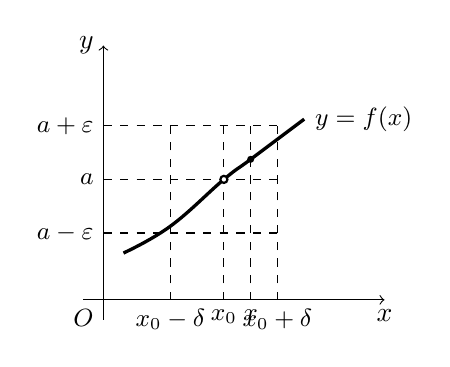
\begin{tikzpicture}[scale=0.85]
  \draw[->] (-0.3,0) -- (4.2,0) node[below] {$x$};
  \draw[->] (0,-0.3) -- (0,3.8) node[left] {$y$};
  \node[below left] at (0,0) {\small $O$};
  
  \draw[dashed] (1.0,0) node[below] {\small $x_0-\delta$} -- (1.0,2.6);
  \draw[dashed] (1.8,0) node[below] {\small $x_0$} -- (1.8,2.6);
  \draw[dashed] (2.2,0) node[below] {\small $x$} -- (2.2,2.6);
  \draw[dashed] (2.6,0) node[below] {\small $x_0+\delta$} -- (2.6,2.6);
  
  \draw[dashed] (0,1.0) node[left] {\small $a-\varepsilon$} -- (2.6,1.0);
  \draw[dashed] (0,1.8) node[left] {\small $a$} -- (2.6,1.8);
  \draw[dashed] (0,2.6) node[left] {\small $a+\varepsilon$} -- (2.6,2.6);
  
  \draw[very thick] plot [smooth, tension=0.7] coordinates {(0.3,0.7) (1.0,1.1) (1.8,1.8) (2.2,2.1) (3.0,2.7)} node[right, font=\small] {$y=f(x)$};
  \fill (2.2,2.1) circle (1.5pt);
  \filldraw[fill=white, draw=black, thick] (1.8,1.8) circle (1.5pt);
\end{tikzpicture}
\caption{}\label{fig:2.1.7}
\end{minipage}
\hfill
\begin{minipage}[t]{0.45\textwidth}
\centering
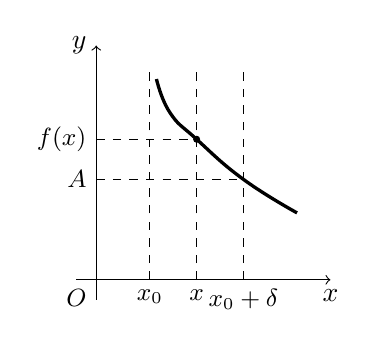
\begin{tikzpicture}[scale=0.85]
  \draw[->] (-0.3,0) -- (3.5,0) node[below] {$x$};
  \draw[->] (0,-0.3) -- (0,3.5) node[left] {$y$};
  \node[below left] at (0,0) {\small $O$};
  
  \draw[dashed] (0.8,0) node[below] {\small $x_0$} -- (0.8,3.2);
  \draw[dashed] (1.5,0) node[below] {\small $x$} -- (1.5,3.2);
  \draw[dashed] (2.2,0) node[below] {\small $x_0+\delta$} -- (2.2,3.2);
  
  \draw[dashed] (0,1.5) node[left] {\small $A$} -- (2.2,1.5);
  \draw[dashed] (0,2.1) node[left] {\small $f(x)$} -- (1.5,2.1);
  
  \draw[very thick] plot [smooth, tension=0.8] coordinates {(0.9,3.0) (1.1,2.5) (1.5,2.1) (2.2,1.5) (3.0,1.0)};
  \fill (1.5,2.1) circle (1.5pt);
\end{tikzpicture}
\caption{}\label{fig:2.1.8}
\end{minipage}
\end{figure}

设函数 $y = f(x)$ 在 $\infty$ 的开邻域 $(-\infty, -\Delta_{0}) \cup (\Delta_{0}, +\infty)$ 内有定义. 如果 $\forall A > 0, \exists \Delta > \Delta_{0} > 0$, 当 $|x| > \Delta$ 时, 有
\[
|f(x)|>A,
\]
则称函数 $y = f(x)$ 在 $\infty$ 处(当 $x \to \infty$ 时)有极限 $\infty$, 记作 $f(\infty) = \lim\limits_{x \to \infty} f(x) = \infty$ 或 $f(x) \to \infty\ (x \to \infty)$ (如图~\ref{fig:2.1.9} 所示).

设函数 $y = f(x)$ 在 $+\infty$ 的开邻域 $(\Delta_{0}, +\infty)$ 内有定义. 如果 $\forall \varepsilon > 0, \exists \Delta > \Delta_{0} > 0$, 当 $x > \Delta$ 时, 有
\[
|f(x)-a|<\varepsilon,
\]
则称函数 $y = f(x)$ 在 $+\infty$ 处(当 $x \to +\infty$ 时)有极限 $a$, 记作 $\lim\limits_{x \to +\infty} f(x) = a$ 或 $f(x) \to a\ (x \to +\infty)$ (如图~\ref{fig:2.1.10} 所示).

\begin{figure}[htbp]
\centering
\begin{minipage}[t]{0.45\textwidth}
\centering
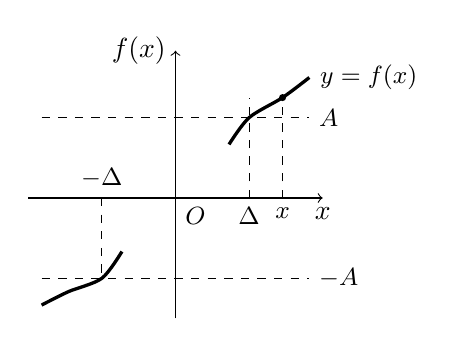
\begin{tikzpicture}[scale=0.85]
  \draw[->] (-2.2,0) -- (2.2,0) node[below] {$x$};
  \draw[->] (0,-1.8) -- (0,2.2) node[left] {$f(x)$};
  \node[below right] at (0,0) {\small $O$};
  
  \draw[dashed] (1.1,0) node[below] {\small $\Delta$} -- (1.1,1.5);
  \draw[dashed] (1.6,0) node[below] {\small $x$} -- (1.6,1.5);
  \draw[dashed] (-1.1,0) node[above] {\small $-\Delta$} -- (-1.1,-1.2);
  
  \draw[dashed] (-2,1.2) -- (2,1.2) node[right] {\small $A$};
  \draw[dashed] (-2,-1.2) -- (2,-1.2) node[right] {\small $-A$};
  
  \draw[very thick] plot [smooth] coordinates {(0.8,0.8) (1.1,1.2) (1.6,1.5) (2.0,1.8)} node[right, font=\small] {$y=f(x)$};
  \draw[very thick] plot [smooth] coordinates {(-2.0,-1.6) (-1.6,-1.4) (-1.1,-1.2) (-0.8,-0.8)};
  \fill (1.6,1.5) circle (1.5pt);
\end{tikzpicture}
\caption{}\label{fig:2.1.9}
\end{minipage}
\hfill
\begin{minipage}[t]{0.45\textwidth}
\centering
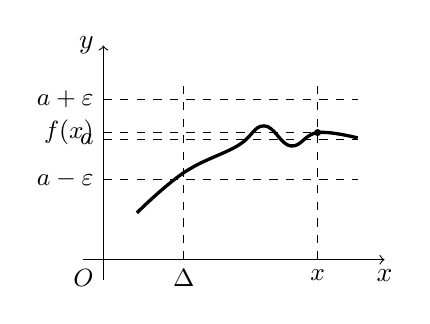
\begin{tikzpicture}[scale=0.85]
  \draw[->] (-0.3,0) -- (4.2,0) node[below] {$x$};
  \draw[->] (0,-0.3) -- (0,3.2) node[left] {$y$};
  \node[below left] at (0,0) {\small $O$};
  
  \draw[dashed] (1.2,0) node[below] {\small $\Delta$} -- (1.2,2.6);
  \draw[dashed] (3.2,0) node[below] {\small $x$} -- (3.2,2.6);
  
  \draw[dashed] (0,1.2) node[left] {\small $a-\varepsilon$} -- (3.8,1.2);
  \draw[dashed] (0,1.8) node[left] {\small $a$} -- (3.8,1.8);
  \draw[dashed] (0,2.4) node[left] {\small $a+\varepsilon$} -- (3.8,2.4);
  \draw[dashed] (0,1.9) node[left] {\small $f(x)$} -- (3.2,1.9);
  
  \draw[very thick] plot [smooth, tension=0.7] coordinates {(0.5,0.7) (1.2,1.3) (2.0,1.7) (2.4,2.0) (2.8,1.7) (3.2,1.9) (3.8,1.82)};
  \fill (3.2,1.9) circle (1.5pt);
\end{tikzpicture}
\caption{}\label{fig:2.1.10}
\end{minipage}
\end{figure}

其余 20 种情形读者自行叙述, 并配出相应的示意图.

\begin{theorem}\label{thm:2.1.1}
$\lim\limits_{x \to x_0} f(x) = a \iff f(x_0^+) = \lim\limits_{x \to x_0^+} f(x) = a = \lim\limits_{x \to x_0^-} f(x) = f(x_0^-)$, 其中 $a$ 为实数, $+\infty, -\infty, \infty$.
\end{theorem}

\begin{proof}
($\Rightarrow$) 显然.

($\Leftarrow$) 对于 $a$ 的任何开邻域 $U(a)$, 因 $\lim\limits_{x\to x_0^+}f(x)=a$, 故 $\exists\delta_1>0$, 当 $x_0<x<x_0+\delta_1$ 时, $f(x)\in U(a)$. 因为 $\lim\limits_{x\to x_0^-}f(x)=a$, 所以 $\exists\delta_2>0$, 当 $x_0-\delta_2<x<x_0$ 时, $f(x)\in U(a)$.

因此, 取 $\delta = \min\{\delta_1, \delta_2\}$, 当 $0 < |x - x_0| < \delta$ 时, 有 $f(x) \in U(a)$. 于是,
\[
\lim_{x\to x_{0}}f(x)=a.
\]
\end{proof}

\begin{theorem}\label{thm:2.1.2}
$\lim\limits_{x\to\infty}f(x)=a \iff \lim\limits_{x\to+\infty}f(x)=a$ 且 $\lim\limits_{x\to-\infty}f(x)=a$, 其中 $a$ 为实数, $+\infty, -\infty, \infty$.
\end{theorem}

\begin{proof}
($\Rightarrow$) 对 $a$ 的任何开邻域 $U(a)$, 因 $\lim\limits_{x\to\infty}f(x)=a$, 故 $\exists\Delta>0$, 当 $|x|>\Delta$ 时, 必有 $f(x)\in U(a)$. 于是, 当 $x>\Delta$ 时, 有 $f(x)\in U(a)$, 从而 $\lim\limits_{x\to+\infty}f(x)=a$; 当 $x < -\Delta$ 时, 有 $f(x) \in U(a)$, 从而 $\lim\limits_{x\to-\infty} f(x) = a$.

($\Leftarrow$) 由 $\lim\limits_{x\to+\infty}f(x)=a$, 故对 $a$ 的任何开邻域 $U(a)$, $\exists\Delta_{1}>0$, 当 $x>\Delta_{1}$ 时, 有 $f(x)\in U(a)$. 再由 $\lim\limits_{x\to-\infty}f(x)=a$, 故对 $a$ 的任何开邻域 $U(a)$, $\exists\Delta_{2}>0$, 当 $x<-\Delta_{2}$ 时, 有 $f(x)\in U(a)$. 因此当 $|x|>\Delta=\max\{\Delta_{1},\Delta_{2}\}$ 时, $f(x)\in U(a)$, 从而 $\lim\limits_{x\to\infty}f(x)=a$.
\end{proof}

\begin{theorem}[归结原则, Heine]\label{thm:2.1.3}
函数 $y = f(x)$, 其定义域为 $x_{0}$ 的去心开邻域 $U^{\circ}(x_{0})$, 则在 $U^{\circ}(x_{0})$ 中有
\[
\lim_{x\to x_0}f(x)=a \iff \forall \{x_n\}\subset U^\circ(x_0),\ x_n\to x_0\ (n\to+\infty),\text{ 必有 } \lim_{n\to+\infty}f(x_n)=a,
\]
其中 $a$ 为实数, $+\infty, -\infty, \infty$; $x_0$ 可换为 $x_0^+, x_0^-, +\infty, -\infty, \infty$.
\end{theorem}

\begin{proof}
先证 $a \in \mathbb{R}, x_0 \in \mathbb{R}$ 的情形.

($\Rightarrow$) $\forall\varepsilon>0$, 因为 $\lim\limits_{x\to x_0}f(x)=a$, 所以 $\exists\delta>0$, 当 $0<|x-x_0|<\delta$ 时, $|f(x)-a|<\varepsilon$. 而由于 $\forall x_n\neq x_0, x_n\to x_0\ (n\to+\infty)$, 所以对取定的 $\delta>0$, $\exists N\in\mathbb{N}$, 当 $n>N$ 时, 有 $0<|x_n-x_0|<\delta$, 所以
\[
|f(x_{n})-a|<\varepsilon,
\]
即 $\lim\limits_{n\to+\infty}f(x_{n})=a$.

($\Leftarrow$) (反证)假设 $\lim\limits_{x \to x_0} f(x) \neq a$, 则 $\exists \varepsilon_0 > 0, \forall n \in \mathbb{N}$, $\exists x_n \neq x_0$, s.t. $0 < |x_n - x_0| < \frac{1}{n}$, 但
\[
|f(x_{n})-a|\geqslant\varepsilon_{0}.
\]
显然, $\lim\limits_{n\to+\infty} x_{n}=x_{0}$, 但由条件知,
\[
0=|a-a|=\lim_{n\to+\infty}|f(x_{n})-a|\geqslant\varepsilon_{0}>0,
\]
矛盾. 所以, $\lim\limits_{x\to x_0}f(x)=a$.

其他情形可类似证明.

统一描述如下:

($\Rightarrow$) 对 $a$ 的任何开邻域 $U(a)$, 因为 $\lim\limits_{x \to x_0} f(x) = a$, 存在 $x_0$ 的去心开邻域 $V^\circ(x_0)$, 当 $x \in V^\circ(x_0)$ 时, $f(x) \in U(a)$. 又因 $x_n \to x_0\ (n \to +\infty), x_n \neq x_0$, 故 $\exists N \in \mathbb{N}$, 当 $n > N$ 时, $x_n \in V^\circ(x_0)$, 从而 $f(x_n) \in U(a)$. 这就证明了 $\lim\limits_{n \to +\infty} f(x_n) = a$.

($\Leftarrow$) (反证)假设 $\lim\limits_{x\to x_0}f(x)\neq a$, 则存在 $a$ 的开邻域 $U_0(a)$, $\forall n\in\mathbb{N}$, $\exists x_n\neq x_0$, s.t. $x_n\in V^\circ_n(x_0)$ (6 种情形分别为 $(x_0-\frac{1}{n},x_0+\frac{1}{n})\setminus\{x_0\}$, $(x_0,x_0+\frac{1}{n})$, $(x_0-\frac{1}{n},x_0)$, $(n,+\infty)$, $(-\infty,-n)$, $(-\infty,-n)\cup(n,+\infty)$), 但是 $f(x_n)\notin U_0(a)$. 显然, $\lim\limits_{n\to+\infty}x_n=x_0$, 但 $\lim\limits_{n\to+\infty}f(x_n)\neq a$, 这与已知条件矛盾.
\end{proof}

\begin{theorem}[函数收敛的 Cauchy 准则]\label{thm:2.1.4}
设 $f$ 在 $x_{0}$ 的去心开邻域 $U^{\circ}(x_{0},\delta_{0})$ 内定义, 则 $\lim\limits_{x\to x_0} f(x)$ 存在有限 $\iff \forall\varepsilon>0,\exists\delta\in(0,\delta_{0})$, s.t. $\forall x^{\prime},x^{\prime\prime}\in U^{\circ}(x_{0},\delta)$, 有
\[
|f(x^{\prime})-f(x^{\prime \prime})|<\varepsilon.
\]
\end{theorem}

\begin{proof}
($\Rightarrow$) 设 $\lim\limits_{x\to x_0}f(x)=a\in\mathbb{R}$, 则 $\forall\varepsilon>0,\exists\delta\in(0,\delta_0)$, s.t. $\forall x\in U^\circ(x_0,\delta)$, 有 $|f(x)-a|<\frac{\varepsilon}{2}$. 于是, 对于 $\forall x',x''\in U^\circ(x_0,\delta)$, 有
\begin{align*}
|f(x^{\prime})-f(x^{\prime \prime})| &= |(f(x^{\prime})-a)-(f(x^{\prime \prime})-a)| \\
&\leqslant |f(x^{\prime})-a|+|f(x^{\prime \prime})-a| < \frac{\varepsilon}{2}+\frac{\varepsilon}{2}=\varepsilon.
\end{align*}

($\Leftarrow$) 设数列 $\{x_n\}\subset U^\circ(x_0,\delta_0)$, 且 $\lim\limits_{n\to+\infty}x_n=x_0$. 按已知条件, $\forall\varepsilon>0$, $\exists\delta\in(0,\delta_0)$, s.t. $\forall x',x''\in U^\circ(x_0,\delta)$, 有 $|f(x')-f(x'')|<\varepsilon$.

对上述的 $\delta$, 由于 $\lim\limits_{n\to+\infty}x_n=x_0$, 故 $\exists N\in\mathbb{N}$, 当 $n,m>N$ 时, 有 $x_n,x_m\in U^\circ(x_0,\delta)$. 从而, $|f(x_n)-f(x_m)|<\varepsilon$. 这表明了 $\{f(x_n)\}$ 为 Cauchy 数列. 根据数列的 Cauchy 准则知, $\{f(x_n)\}$ 收敛.

进一步考虑 $\{x_{n}^{\prime}\}\subset U^{\circ}(x_{0},\delta_{0})$, $\{x_{n}^{\prime\prime}\}\subset U^{\circ}(x_{0},\delta_{0})$, 且 $\lim\limits_{n\to+\infty}x_{n}^{\prime}=x_{0}=\lim\limits_{n\to+\infty}x_{n}^{\prime\prime}$. 构造交错数列 $\{x_n\}\colon x_{1}^{\prime}, x_{1}^{\prime\prime}, x_{2}^{\prime}, x_{2}^{\prime\prime}, \cdots, x_{k}^{\prime}, x_{k}^{\prime\prime}, \cdots$, 显然 $\{x_{n}\}\subset U^{\circ}(x_{0},\delta_{0})$, $\lim\limits_{n\to+\infty}x_{n}=x_{0}$. 由上述证明所得结果, $\{f(x_{n})\}$ 收敛, 从而
\[
\lim_{n\to+\infty}f(x_{n}^{\prime})=\lim_{n\to+\infty}f(x_{n})=\lim_{n\to+\infty}f(x_{n}^{\prime\prime}),
\]
记此公共极限为 $a$. 根据归结原则(定理~\ref{thm:2.1.3}), $\lim\limits_{x\to x_0}f(x)=a$.
\end{proof}

\begin{remark}\label{rem:2.1.1}
定理~\ref{thm:2.1.4} 等价于: $f(x)$ 在 $x_{0}$ 不存在有限极限 $\iff \exists \varepsilon_{0} > 0, \forall \delta > 0$, 总有 $x_{\delta}^{\prime}, x_{\delta}^{\prime\prime} \in U^{\circ}(x_{0}, \delta)$, s.t. $|f(x_{\delta}^{\prime}) - f(x_{\delta}^{\prime\prime})| \geqslant \varepsilon_{0}$.
\end{remark}

\begin{remark}\label{rem:2.1.2}
定理~\ref{thm:2.1.4} 与注~\ref{rem:2.1.1} 中, $x_{0}$ 换为 $x_{0}^{\pm}, \pm\infty, \infty$, 相应结论成立, 证明也类似.
\end{remark}

\begin{example}\label{ex:2.1.4}
设 $f(x) = c$ 为常值函数, 则 $\lim\limits_{x \to x_0} f(x) = c$, 其中 $x_0$ 或 $x_0^+, x_0^-, +\infty, -\infty, \infty$.
\end{example}

\begin{proof}
$\forall\varepsilon>0$, 任取 $\delta>0$, 当 $0<|x-x_{0}|<\delta$ 时, 有
\[
|f(x)-c|=|c-c|=0<\varepsilon,
\]
所以 $\lim\limits_{x\to x_0}f(x)=c$. 其他情形类似证明.
\end{proof}

\begin{example}\label{ex:2.1.5}
证明: $\lim\limits_{x\to+\infty}\frac{1}{x^\alpha}=0\ (\alpha>0)$.
\end{example}

\begin{proof}
$\forall\varepsilon>0$, 取 $\Delta>\left(\frac{1}{\varepsilon}\right)^{\frac{1}{\alpha}}$, 则当 $x>\Delta$ 时, 有
\[
\left|\frac{1}{x^{\alpha}}-0\right|=\frac{1}{x^{\alpha}}<\frac{1}{\Delta^{\alpha}}<\varepsilon,
\]
所以 $\lim\limits_{x\to+\infty}\frac{1}{x^{\alpha}}=0$.
\end{proof}

\begin{example}\label{ex:2.1.6}
证明:
\begin{enumerate}[label=(\arabic*)]
  \item $\lim\limits_{x\to-\infty}\arctan x=-\frac{\pi}{2}$;
  \item $\lim\limits_{x \to +\infty} \arctan x = \frac{\pi}{2}$.
\end{enumerate}
\end{example}

\begin{proof}
(1) $\forall\varepsilon>0$, 取 $\Delta>\tan\left(\frac{\pi}{2}-\varepsilon\right)$, 当 $x<-\Delta$ 时, 有
\[
-\frac{\pi}{2}-\varepsilon<-\frac{\pi}{2}<\arctan x<\arctan(-\Delta)=-\left(\frac{\pi}{2}-\varepsilon\right)<-\frac{\pi}{2}+\varepsilon,
\]
因此 $\lim\limits_{x\to-\infty}\arctan x=-\frac{\pi}{2}$.

(2) $\forall\varepsilon>0$, 取 $\Delta>\tan\left(\frac{\pi}{2}-\varepsilon\right)=\cot\varepsilon$, 当 $x>\Delta$ 时, 有
\[
\frac{\pi}{2}-\varepsilon < \arctan\Delta < \arctan x < \frac{\pi}{2} < \frac{\pi}{2}+\varepsilon,
\]
所以 $\lim\limits_{x\to+\infty}\arctan x=\frac{\pi}{2}$ (如图~\ref{fig:2.1.11} 所示).
\end{proof}

\begin{figure}[htbp]
\centering
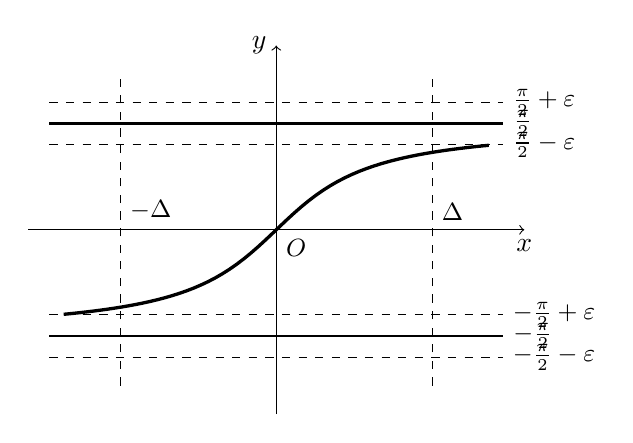
\begin{tikzpicture}[scale=0.9]
  \draw[->] (-3.5,0) -- (3.5,0) node[below] {$x$};
  \draw[->] (0,-2.6) -- (0,2.6) node[left] {$y$};
  \node[below right] at (0,0) {\small $O$};
  
  \draw[thick] (-3.2,1.5) -- (3.2,1.5) node[right] {\small $\frac{\pi}{2}$};
  \draw[thick] (-3.2,-1.5) -- (3.2,-1.5) node[right] {\small $-\frac{\pi}{2}$};
  
  \draw[dashed] (-3.2,1.8) -- (3.2,1.8) node[right] {\small $\frac{\pi}{2}+\varepsilon$};
  \draw[dashed] (-3.2,1.2) -- (3.2,1.2) node[right] {\small $\frac{\pi}{2}-\varepsilon$};
  \draw[dashed] (-3.2,-1.2) -- (3.2,-1.2) node[right] {\small $-\frac{\pi}{2}+\varepsilon$};
  \draw[dashed] (-3.2,-1.8) -- (3.2,-1.8) node[right] {\small $-\frac{\pi}{2}-\varepsilon$};
  
  \draw[dashed] (2.2,-2.2) -- (2.2,2.2);
  \node[above right] at (2.2,0) {\small $\Delta$};
  \draw[dashed] (-2.2,-2.2) -- (-2.2,2.2);
  \node[above right] at (-2.2,0) {\small $-\Delta$};
  
  \draw[very thick, domain=-3:3, samples=60] plot (\x, {1.5*(2/pi)*rad(atan(\x))});
\end{tikzpicture}
\caption{}\label{fig:2.1.11}
\end{figure}

\begin{example}\label{ex:2.1.7}
证明: $\lim\limits_{x\to2}\frac{x^{2}-4}{x-2}=\lim\limits_{x\to2}(x+2)=4$.
\end{example}

\begin{proof}
$\forall\varepsilon>0$, 取 $\delta=\varepsilon$, 当 $0<|x-2|<\delta=\varepsilon$ 时, 有
\[
\left|\frac{x^{2}-4}{x-2}-4\right|=|(x+2)-4|=|x-2|<\delta=\varepsilon,
\]
因此 $\lim\limits_{x\to2}\frac{x^{2}-4}{x-2}=4$.
\end{proof}

函数 $y=\frac{x^{2}-4}{x-2}$ 和 $y=x+2$ 的定义域不同, 前者为 $\mathbb{R}\setminus\{2\}$, 后者为 $\mathbb{R}$, 但它们在 $x\to2$ 时有相同的极限, 这是因为在考虑 $x\to x_{0}$ 的极限时, 并不要求函数在 $x=x_{0}$ 处有定义或函数在 $x_{0}$ 处的值是多少. 下面的例子也是如此.

\begin{example}\label{ex:2.1.8}
证明: $\lim\limits_{x\to1}\frac{x^{2}-1}{2x^{2}-x-1}=\lim\limits_{x\to1}\frac{x+1}{2x+1}=\frac{2}{3}$.
\end{example}

\begin{proof}
$\forall\varepsilon>0$, 取 $\delta=\min\{1,3\varepsilon\}$ (如图~\ref{fig:2.1.12} 所示), 当 $0<|x-1|<\delta$ 时, 有
\[
\left|\frac{x^2-1}{2x^2-x-1}-\frac{2}{3}\right|=\left|\frac{x+1}{2x+1}-\frac{2}{3}\right|=\frac{|x-1|}{3|2x+1|}<\frac{\delta}{3}\leqslant\varepsilon,
\]
所以 $\lim\limits_{x\to1}\frac{x^{2}-1}{2x^{2}-x-1}=\frac{2}{3}$.
\end{proof}

\begin{remark}\label{rem:2.1.3}
为了使得 $|2x+1|\geqslant1$, 我们先限制 $|x-1|<1\iff 0<x<2$. 再由 $\frac{\delta}{3}\leqslant\varepsilon$ 解得 $\delta\leqslant3\varepsilon$, 所以取 $\delta=\min\{1,3\varepsilon\}$.

如果先限制 $|x-1| < \frac{1}{2} \iff -\frac{1}{2} < x-1 < \frac{1}{2} \iff \frac{1}{2} < x < \frac{3}{2}$ (如图~\ref{fig:2.1.13} 所示). 于是, $|2x+1| \geqslant |2 \cdot \frac{1}{2}+1| = 2$, 从而
\[
\left|\frac{x^{2}-1}{2x^{2}-x-1}-\frac{2}{3}\right|=\frac{|x-1|}{3|2x+1|}<\frac{\delta}{3\cdot2}=\frac{\delta}{6}\leqslant\varepsilon,
\]
只需取 $\delta = \min\left\{\frac{1}{2},6\varepsilon\right\}$.
\end{remark}

\begin{figure}[htbp]
\centering
\begin{minipage}[t]{0.45\textwidth}
\centering
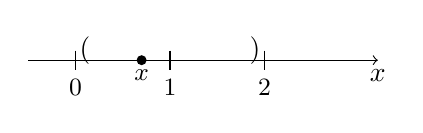
\begin{tikzpicture}[scale=1.2]
  \draw[->] (-0.5,0) -- (3.2,0) node[below] {$x$};
  \draw (0,0.1) -- (0,-0.1) node[below] {\small $0$};
  \draw (1,0.1) -- (1,-0.1) node[below] {\small $1$};
  \draw (2,0.1) -- (2,-0.1) node[below] {\small $2$};
  \node at (0.1,0.1) {$($};
  \node at (1.9,0.1) {$)$};
  \fill (0.7,0) circle (1.5pt) node[below] {\small $x$};
\end{tikzpicture}
\caption{}\label{fig:2.1.12}
\end{minipage}
\hfill
\begin{minipage}[t]{0.45\textwidth}
\centering
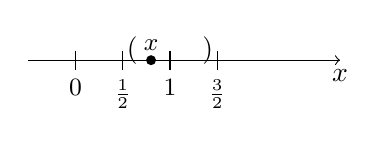
\begin{tikzpicture}[scale=1.2]
  \draw[->] (-0.5,0) -- (2.8,0) node[below] {$x$};
  \draw (0,0.1) -- (0,-0.1) node[below] {\small $0$};
  \draw (0.5,0.1) -- (0.5,-0.1) node[below] {\small $\frac{1}{2}$};
  \draw (1,0.1) -- (1,-0.1) node[below] {\small $1$};
  \draw (1.5,0.1) -- (1.5,-0.1) node[below] {\small $\frac{3}{2}$};
  \node at (0.6,0.1) {$($};
  \node at (1.4,0.1) {$)$};
  \fill (0.8,0) circle (1.5pt) node[above] {\small $x$};
\end{tikzpicture}
\caption{}\label{fig:2.1.13}
\end{minipage}
\end{figure}

\begin{example}\label{ex:2.1.9}
证明:
\begin{enumerate}[label=(\arabic*)]
  \item $\lim\limits_{x\to1^{+}}\frac{x^{2}+1}{x^{2}-1}=+\infty$;
  \item $\lim\limits_{x \to 1^-} \frac{x^2 + 1}{x^2 - 1} = -\infty$.
\end{enumerate}
\end{example}

\begin{proof}
(1) $\forall A>0$, 取 $\delta=\min\left\{1,\frac{1}{3A}\right\}$ (如图~\ref{fig:2.1.14} 所示), 当 $1<x<1+\delta$ 时, 有
\[
\frac{x^{2}+1}{x^{2}-1}=\frac{x^{2}+1}{(x+1)(x-1)}>\frac{1}{(2+1)\delta}=\frac{1}{3\delta}\geqslant A,
\]
所以 $\lim\limits_{x\to1^{+}}\frac{x^{2}+1}{x^{2}-1}=+\infty$.

(2) $\forall A>0$, 取 $\delta=\min\left\{1,\frac{1}{2A}\right\}$ (如图~\ref{fig:2.1.15} 所示), 当 $1-\delta<x<1$ 时, 有
\[
\frac{x^{2}+1}{x^{2}-1}=\frac{x^{2}+1}{(x+1)(x-1)}=-\frac{x^{2}+1}{(x+1)(1-x)}<-\frac{1}{2\delta}<-A,
\]
因此 $\lim\limits_{x\to1^{-}}\frac{x^{2}+1}{x^{2}-1}=-\infty$.
\end{proof}

\begin{figure}[htbp]
\centering
\begin{minipage}[t]{0.45\textwidth}
\centering
\begin{tikzpicture}[scale=1.2]
  \draw[->] (-0.5,0) -- (3.2,0) node[below] {$x$};
  \draw (0,0.1) -- (0,-0.1) node[below] {\small $0$};
  \draw (1,0.1) -- (1,-0.1) node[below] {\small $1$};
  \draw (2,0.1) -- (2,-0.1) node[below] {\small $2$};
  \node at (1.8,0.1) {$)$};
  \fill (1.4,0) circle (1.5pt) node[below] {\small $x$};
\end{tikzpicture}
\caption{}\label{fig:2.1.14}
\end{minipage}
\hfill
\begin{minipage}[t]{0.45\textwidth}
\centering
\begin{tikzpicture}[scale=1.2]
  \draw[->] (-0.5,0) -- (3.2,0) node[below] {$x$};
  \draw (0,0.1) -- (0,-0.1) node[below] {\small $0$};
  \draw (1,0.1) -- (1,-0.1) node[below] {\small $1$};
  \draw (2,0.1) -- (2,-0.1) node[below] {\small $2$};
  \node at (0.2,0.1) {$($};
  \fill (0.7,0) circle (1.5pt) node[below] {\small $x$};
\end{tikzpicture}
\caption{}\label{fig:2.1.15}
\end{minipage}
\end{figure}

\begin{example}\label{ex:2.1.10}
证明 $\lim\limits_{x\to0}x^{\alpha}\sin\frac{1}{x}=0\ (\alpha>0)$ (如图~\ref{fig:2.1.16} 所示).
\end{example}

\begin{proof}
$\forall\varepsilon>0$, 取 $\delta=\varepsilon^{\frac{1}{\alpha}}$, 当 $0<|x-0|<\delta$ 时, 有
\[
\left|x^{\alpha}\sin\frac{1}{x}-0\right|\leqslant|x|^{\alpha}<\delta^{\alpha}=\varepsilon,
\]
这就证明了 $\lim\limits_{x\to0}x^{\alpha}\sin\frac{1}{x}=0$.
\end{proof}

\begin{figure}[htbp]
\centering
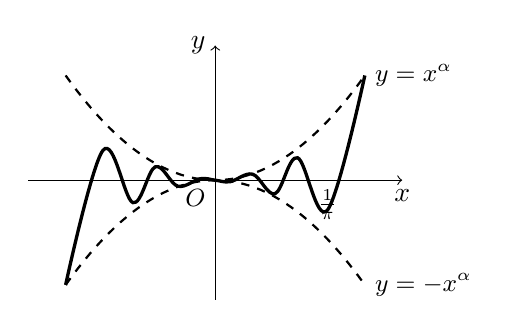
\begin{tikzpicture}[scale=0.95]
  \draw[->] (-2.5,0) -- (2.5,0) node[below] {$x$};
  \draw[->] (0,-1.6) -- (0,1.8) node[left] {$y$};
  \node[below left] at (0,0) {\small $O$};
  
  \draw[dashed, thick, domain=-2:2, samples=50] plot (\x, {0.35*\x*\x}) node[right] {\small $y=x^\alpha$};
  \draw[dashed, thick, domain=-2:2, samples=50] plot (\x, {-0.35*\x*\x}) node[right] {\small $y=-x^\alpha$};
  
  \draw[very thick] plot [smooth, tension=0.6] coordinates {
    (-2.0, -1.4) (-1.5, 0.4) (-1.1, -0.3) (-0.8, 0.18) (-0.5, -0.08) (-0.2, 0.02)
    (0,0)
    (0.2, -0.02) (0.5, 0.08) (0.8, -0.18) (1.1, 0.3) (1.5, -0.4) (2.0, 1.4)
  };
  \node[below] at (1.5,0) {\small $\frac{1}{\pi}$};
\end{tikzpicture}
\caption{}\label{fig:2.1.16}
\end{figure}

\begin{example}\label{ex:2.1.11}
设 $\lim\limits_{x\to x_0}f(x)=0, |g(x)|\leqslant M$, 则 $\lim\limits_{x\to x_0}f(x)g(x)=0$.
\end{example}

\begin{proof}
$\forall\varepsilon>0$, 因 $\lim\limits_{x\to x_0}f(x)=0$, 故 $\exists\delta>0$, 当 $0<|x-x_0|<\delta$ 时, 有 $|f(x)-0|<\frac{\varepsilon}{M+1}$. 于是,
\[
|f(x)g(x)-0|=|f(x)|\cdot|g(x)|\leqslant M|f(x)-0|<M\cdot\frac{\varepsilon}{M+1}<\varepsilon,
\]
这就证明了 $\lim\limits_{x\to x_{0}}f(x)g(x)=0$.
\end{proof}

\begin{example}\label{ex:2.1.12}
设
\[
f(x)=\begin{cases}
1, & x<0, \\
x\sin\frac{1}{x}, & x>0.
\end{cases}
\]
证明: $\lim\limits_{x\to0}f(x)$ 不存在.
\end{example}

\begin{proof}
因为
\begin{align*}
f(0+0) &= f(0^{+})=\lim_{x\to0^{+}}x\sin\frac{1}{x}=0, \\
f(0-0) &= f(0^{-})=\lim_{x\to0^{-}}f(x)=\lim_{x\to0^{-}}1=1,
\end{align*}
$f(0^{+})\neq f(0^{-})$, 所以根据定理~\ref{thm:2.1.1} 知, $\lim\limits_{x\to0}f(x)$ 不存在.
\end{proof}

\begin{example}\label{ex:2.1.13}
证明: 符号函数 $\operatorname{sgn} x$ 在 $x=0$ 处无极限.
\end{example}

\begin{proof}
因为
\[
\operatorname{sgn}(0^{+})=\lim_{x\to0^{+}}\operatorname{sgn} x=\lim_{x\to0^{+}}1=1\neq-1=\lim_{x\to0^{-}}(-1)=\lim_{x\to0^{-}}\operatorname{sgn} x=\operatorname{sgn}(0^{-}),
\]
所以根据定理~\ref{thm:2.1.1} 知, $\operatorname{sgn} x$ 在 $x=0$ 处无极限.
\end{proof}

\begin{example}\label{ex:2.1.14}
证明 $\lim\limits_{x\to0}\sin\frac{1}{x}$ 不存在.
\end{example}

\begin{proof}
取数列 $x_{n}^{\prime}=\frac{1}{2n\pi}\to0\ (n\to+\infty)$, $x_{n}^{\prime\prime}=\frac{1}{2n\pi+\frac{\pi}{2}}\to0\ (n\to+\infty)$. 显然,
\begin{align*}
\lim_{n\to+\infty}\sin\frac{1}{x_{n}^{\prime}} &= \lim_{n\to+\infty}\sin 2n\pi = 0, \\
\lim_{n\to+\infty}\sin\frac{1}{x_{n}^{\prime\prime}} &= \lim_{n\to+\infty}\sin\left(2n\pi+\frac{\pi}{2}\right) = 1,
\end{align*}
$\lim\limits_{n\to+\infty}\sin\frac{1}{x_{n}^{\prime}}\neq\lim\limits_{n\to+\infty}\sin\frac{1}{x_{n}^{\prime\prime}}$. 所以根据定理~\ref{thm:2.1.3} 知, $\lim\limits_{x\to0}\sin\frac{1}{x}$ 不存在(如图~\ref{fig:2.1.17} 所示).
\end{proof}

\begin{figure}[htbp]
\centering
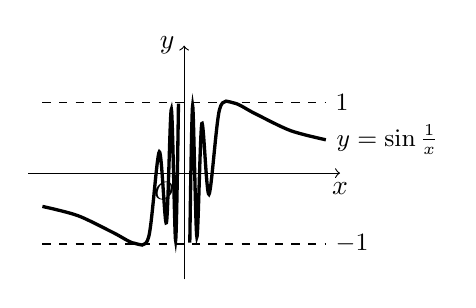
\begin{tikzpicture}[scale=0.9]
  \draw[->] (-2.2,0) -- (2.2,0) node[below] {$x$};
  \draw[->] (0,-1.5) -- (0,1.8) node[left] {$y$};
  \node[below left] at (0,0) {\small $O$};
  
  \draw[dashed] (-2,1) -- (2,1) node[right] {\small $1$};
  \draw[dashed] (-2,-1) -- (2,-1) node[right] {\small $-1$};
  
  \draw[very thick] plot [smooth, tension=0.5] coordinates {
    (-2.0,-0.47) (-1.5,-0.6) (-1.0,-0.84) (-0.7,-0.99) (-0.5,-0.9)
    (-0.35, 0.3) (-0.25, -0.7) (-0.18, 0.9) (-0.12, -0.95) (-0.08, 0.98)
  };
  \draw[very thick] plot [smooth, tension=0.5] coordinates {
    (0.08, -0.98) (0.12, 0.95) (0.18, -0.9) (0.25, 0.7) (0.35, -0.3)
    (0.5, 0.9) (0.7, 0.99) (1.0, 0.84) (1.5, 0.6) (2.0, 0.47)
  } node[right, font=\small] {$y=\sin\frac{1}{x}$};
\end{tikzpicture}
\caption{}\label{fig:2.1.17}
\end{figure}

\begin{example}\label{ex:2.1.15}
证明 Dirichlet 函数
\[
D(x)=\begin{cases}
1, & x\in\mathbb{Q}, \\
0, & x\in\mathbb{R}\setminus\mathbb{Q}
\end{cases}
\]
在任何点处无极限.
\end{example}

\begin{proof}
\textit{证法 1}\quad $\forall x_0 \in \mathbb{R}$, 取 $x'_n \in \mathbb{Q}, x'_n \neq x_0, x'_n \to x_0\ (n \to +\infty)$; 再取 $x''_n \in \mathbb{R} \setminus \mathbb{Q}, x''_n \neq x_0, x''_n \to x_0\ (n \to +\infty)$, 则
\[
\lim_{n\to+\infty}D(x_{n}^{\prime})=\lim_{n\to+\infty}1=1,\quad \lim_{n\to+\infty}D(x_{n}^{\prime \prime})=\lim_{n\to+\infty}0=0.
\]
因为 $\lim\limits_{n\to+\infty}D(x_{n}^{\prime})\neq\lim\limits_{n\to+\infty}D(x_{n}^{\prime\prime})$, 所以根据定理~\ref{thm:2.1.3} 知, $\lim\limits_{x\to x_{0}}D(x)$ 不存在.

\textit{证法 2}\quad (反证)反设在点 $x_{0} \in \mathbb{R}$, $\lim\limits_{x \to x_{0}} D(x) = a$, 则 $0$ 与 $1$ 中至少有一个不为 $a$. 不妨设 $a \neq 1$, 则存在 $a$ 的开邻域 $U(a) \not\ni 1$. 于是, $\exists \delta > 0$, 当 $0 < |x - x_{0}| < \delta$ 时, $D(x) \in U(a)$, 当然 $D(x) \neq 1$. 但因 $\mathbb{Q}$ 在 $\mathbb{R}$ 中是稠密的, 必有 $x' \in \mathbb{Q}$, s.t. $0 < |x' - x_{0}| < \delta$, 所以 $1=D(x^{\prime})\in U(a)$, 这与 $1 \notin U(a)$ 相矛盾.
\end{proof}

\begin{example}\label{ex:2.1.16}
证明:
\[
\lim_{x\to+\infty}a^x=\begin{cases}
+\infty, & a>1, \\
1, & a=1, \\
0, & 0<a<1.
\end{cases}
\]
\end{example}

\begin{proof}
当 $a>1$ 时, $\forall A>0$, 取 $\Delta>\log_{a}A$. 当 $x>\Delta$ 时, 有
\[
a^{x}>a^{\Delta}>A,
\]
所以 $\lim\limits_{x\to+\infty}a^{x}=+\infty$.

当 $0 < a < 1$ 时, $\forall \varepsilon > 0$, 取 $\Delta > \log_{a}\varepsilon$. 当 $x > \Delta$ 时, 有
\[
|a^{x}-0|=a^{x}<a^{\Delta}<\varepsilon,
\]
所以 $\lim\limits_{x\to+\infty}a^{x}=0$.

当 $a=1$ 时, $\lim\limits_{x\to+\infty}a^{x}=\lim\limits_{x\to+\infty}1^{x}=\lim\limits_{x\to+\infty}1=1$.
\end{proof}

\begin{example}\label{ex:2.1.17}
证明:
\begin{enumerate}[label=(\arabic*)]
  \item $\lim\limits_{x\to 0}a^{x}=1\ (a>0)$;
  \item $\lim\limits_{x \to 1} \log_a x = 0\ (a > 0, a \neq 1)$.
\end{enumerate}
\end{example}

\begin{proof}
(1) 设 $a=1$, 显然 $\lim\limits_{x\to0}a^{x}=\lim\limits_{x\to0}1^{x}=1$.

设 $a>1$. $\forall\varepsilon\in(0,1)$, 取 $\delta=\min\{|\log_{a}(1-\varepsilon)|,|\log_{a}(1+\varepsilon)|\}$, 当 $0<|x-0|=|x|<\delta$ 时, 有
\[
\log_{a}(1-\varepsilon)<x<\log_{a}(1+\varepsilon)\implies 1-\varepsilon<a^{x}<1+\varepsilon\implies |a^{x}-1|<\varepsilon,
\]
所以 $\lim\limits_{x\to0} a^x = 1$.

设 $0 < a < 1$. $\forall \varepsilon \in (0,1)$, 取 $\delta = \min\{|\log_{a}(1-\varepsilon)|, |\log_{a}(1+\varepsilon)|\}$, 当 $0 < |x| < \delta$ 时, 有
\[
\log_{a}(1+\varepsilon)<x<\log_{a}(1-\varepsilon)\implies 1-\varepsilon<a^{x}<1+\varepsilon\implies |a^{x}-1|<\varepsilon,
\]
所以 $\lim\limits_{x\to0}a^{x}=1$.

(2) 不失一般性, 设 $a > 1$. $\forall \varepsilon > 0$, 必存在 $\varepsilon_{1} > 0$, 使得 $a^{-\varepsilon} < 1 - \varepsilon_{1} < 1 + \varepsilon_{1} < a^{\varepsilon}$. 当 $a^{-\varepsilon}<1-\varepsilon_{1}<x<1+\varepsilon_{1}<a^{\varepsilon}$ 时, 有
\[
-\varepsilon<\log_{a}x<\varepsilon\implies |\log_{a}x-0|<\varepsilon,
\]
故 $\lim\limits_{x\to1}\log_{a}x=0$.
\end{proof}

\begin{lemma}\label{lem:2.1.1}
证明:
\begin{enumerate}[label=(\arabic*)]
  \item $\sin x < x < \tan x,\ 0 < x < \frac{\pi}{2}$;
  \item $\sin x < x,\ \forall x \in (0, +\infty)$;
  \item $|\sin x|\leqslant|x|,\ \forall x\in\mathbb{R}$.
\end{enumerate}
\end{lemma}

\begin{proof}
(1) 图~\ref{fig:2.1.18} 所示是一单位圆, 用 $S_{\triangle OCD}, S_{\text{扇形}OAD}, S_{\triangle OAB}$ 分别表示 $\triangle OCD$, 扇形 $OAD$ 和 $\triangle OAB$ 的面积. 显然,
\[
S_{\triangle OCD}<S_{\text{扇形}OAD}<S_{\triangle OAB},
\]
从而 $\frac{1}{2}\sin x\cos x < \frac{1}{2}x < \frac{1}{2}\tan x$, 于是 $\sin x<x<\tan x\ (0<x<\frac{\pi}{2})$.

\begin{figure}[htbp]
\centering
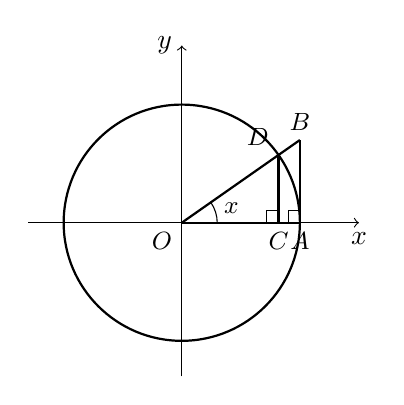
\begin{tikzpicture}[scale=1.5]
  \draw[->] (-1.3,0) -- (1.5,0) node[below] {$x$};
  \draw[->] (0,-1.3) -- (0,1.5) node[left] {$y$};
  \node[below left] at (0,0) {\small $O$};
  
  \draw[thick] (0,0) circle (1cm);
  
  \coordinate (O) at (0,0);
  \coordinate (A) at (1,0);
  \coordinate (D) at ({cos(35)}, {sin(35)});
  \coordinate (C) at ({cos(35)}, 0);
  \coordinate (B) at (1, {tan(35)});
  
  \draw[thick] (O) -- (B);
  \draw[thick] (A) -- (B);
  \draw[thick] (C) -- (D);
  \draw[thick] (O) -- (A);
  
  \node[below] at (A) {\small $A$};
  \node[above] at (B) {\small $B$};
  \node[above left] at (D) {\small $D$};
  \node[below] at (C) {\small $C$};
  
  \draw (0.3,0) arc (0:35:0.3);
  \node at (0.42,0.12) {\small $x$};
  
  \draw (0.9,0) -- (0.9,0.1) -- (1,0.1);
  \draw ({cos(35)},0.1) -- ({cos(35)-0.1},0.1) -- ({cos(35)-0.1},0);
\end{tikzpicture}
\caption{}\label{fig:2.1.18}
\end{figure}

(2) 当 $x \geqslant \frac{\pi}{2}$ 时, $x \geqslant \frac{\pi}{2} > 1 \geqslant \sin x$, 因此 $\sin x<x,\ \forall x\in(0,+\infty)$.

当 $x<0$ 时, $|\sin x|=|\sin(-x)|<-x=|x|$. 结合 $x=0$ 处等号成立, 故 $|\sin x|\leqslant|x|,\ \forall x\in\mathbb{R}$.
\end{proof}

\begin{example}\label{ex:2.1.18}
证明:
\begin{enumerate}[label=(\arabic*)]
  \item $\lim\limits_{x \to x_0} \sin x = \sin x_0$;
  \item $\lim\limits_{x \to x_0} \cos x = \cos x_0\ (x_0 \in \mathbb{R})$.
\end{enumerate}
\end{example}

\begin{proof}
(1) $\forall\varepsilon>0$, 取 $\delta=\varepsilon$, 当 $|x-x_{0}|<\delta$ 时, 由和差化积公式与引理~\ref{lem:2.1.1} 有
\[
|\sin x-\sin x_{0}|=2\left|\cos\frac{x+x_{0}}{2}\right|\left|\sin\frac{x-x_{0}}{2}\right|\leqslant2\left|\frac{x-x_{0}}{2}\right|=|x-x_{0}|<\delta=\varepsilon,
\]
所以 $\lim\limits_{x\to x_0}\sin x=\sin x_0$.

(2) 同理, $\forall\varepsilon>0$, 取 $\delta=\varepsilon$, 当 $|x-x_{0}|<\delta$ 时, 有
\[
|\cos x-\cos x_{0}|=2\left|\sin\frac{x+x_{0}}{2}\right|\left|\sin\frac{x-x_{0}}{2}\right|\leqslant2\left|\frac{x-x_{0}}{2}\right|<\delta=\varepsilon,
\]
所以 $\lim\limits_{x\to x_0}\cos x=\cos x_0$. 或由 $\lim\limits_{x\to x_0}\cos x=\lim\limits_{x\to x_0}\sin\left(\frac{\pi}{2}-x\right)=\sin\left(\frac{\pi}{2}-x_0\right)=\cos x_0$.
\end{proof}

\begin{example}\label{ex:2.1.19}
证明: $\lim\limits_{x\to x_0}\sqrt{x}=\sqrt{x_0}\ (x_0\geqslant0)$.
\end{example}

\begin{proof}
当 $x_{0}=0$ 时, $\forall\varepsilon>0$, 取 $\delta=\varepsilon^{2}$, 当 $0<x<\delta$ 时, 有
\[
|\sqrt{x}-\sqrt{0}|=\sqrt{x}<\sqrt{\delta}=\varepsilon,
\]
故 $\lim\limits_{x\to0^{+}}\sqrt{x}=0$.

当 $x_{0}>0$ 时, 取 $\delta=\min\{x_{0},\sqrt{x_{0}}\varepsilon\}$, 当 $|x-x_{0}|<\delta$ 时, 有
\[
|\sqrt{x}-\sqrt{x_{0}}|=\frac{|x-x_{0}|}{\sqrt{x}+\sqrt{x_{0}}}\leqslant\frac{|x-x_{0}|}{\sqrt{x_{0}}}<\frac{\delta}{\sqrt{x_{0}}}\leqslant\varepsilon,
\]
所以 $\lim\limits_{x\to x_0}\sqrt{x}=\sqrt{x_0}$.
\end{proof}

\begin{example}\label{ex:2.1.20}
证明: $\lim\limits_{x\to\infty}\sqrt{\frac{x^{2}+1}{x^{2}-1}}=1$.
\end{example}

\begin{proof}
\textit{证法 1}\quad $\forall\varepsilon>0$, 取 $\Delta>\max\left\{\sqrt{2},\frac{2}{\varepsilon}\right\}$, 当 $|x|>\Delta$ 时, 有
\begin{align*}
\left|\sqrt{\frac{x^2+1}{x^2-1}}-1\right| &= \left|\frac{\sqrt{x^2+1}-\sqrt{x^2-1}}{\sqrt{x^2-1}}\right|=\frac{2}{\sqrt{x^2-1}(\sqrt{x^2+1}+\sqrt{x^2-1})} \\
&< \frac{2}{x^2-1} \leqslant \frac{2}{\frac{1}{2}x^2} = \frac{4}{x^2} < \varepsilon,
\end{align*}
或放大为 $\frac{2}{|x|} < \frac{2}{\Delta} < \varepsilon$. 所以 $\lim\limits_{x\to\infty}\sqrt{\frac{x^{2}+1}{x^{2}-1}}=1$.

\textit{证法 2}\quad 变形为
\[
\lim_{x\to\infty}\sqrt{\frac{x^{2}+1}{x^{2}-1}}=\lim_{x\to\infty}\sqrt{\frac{1+\frac{1}{x^{2}}}{1-\frac{1}{x^{2}}}}=\sqrt{\frac{1+0}{1-0}}=1.
\]
\end{proof}

\begin{exblock}{练习题 2.1}
  \item 在定义~\ref{def:2.1.3} 中就 24 种情形给出函数极限的定义, 并配出相应的图形.
  \item 按函数极限的定义证明:
  \begin{enumerate}[label=(\arabic*)]
    \item $\lim\limits_{x \to +\infty} \frac{6x + 5}{x} = 6$;
    \item $\lim\limits_{x \to 2} (x^2 - 6x + 10) = 2$;
    \item $\lim\limits_{x \to +\infty} \frac{x^2 - 5}{x^2 - 1} = 1$;
    \item $\lim\limits_{x \to 2^-} \sqrt{4 - x^2} = 0$;
    \item $\lim\limits_{x \to 1} \frac{x^4 - 1}{x - 1} = 4$;
    \item $\lim\limits_{x \to 3} \frac{x - 3}{x^2 - 9} = \frac{1}{6}$;
    \item $\lim\limits_{x\to1^{+}}\frac{x-1}{\sqrt{x^{2}-1}}=0$;
    \item $\lim\limits_{x \to +\infty} (\sqrt{x+1} - \sqrt{x-1}) = 0$;
    \item $\lim\limits_{x \to \infty} \sqrt{\frac{x^2 + 2}{x^2 - 2}} = 1$.
  \end{enumerate}
  \item 设 $\lim\limits_{x \to x_0} f(x) = a$. 用 $\varepsilon - \delta$ 法证明:
  \begin{enumerate}[label=(\arabic*)]
    \item $\lim\limits_{x \to x_0} f^2(x) = a^2$;
    \item $\lim\limits_{x \to x_0} \sqrt{f(x)} = \sqrt{a}\ (a > 0)$;
    \item $\lim\limits_{x \to x_0} \sqrt[3]{f(x)} = \sqrt[3]{a}$.
  \end{enumerate}
  \item 设 $\lim\limits_{x \to x_0} f(x) = a$. 证明: $\lim\limits_{x \to x_0} |f(x)| = |a|$. 举例说明反之不成立. 问: 当且仅当 $a$ 为何值时反之也成立?
  \item 讨论下列函数在点 $0$ 处的极限或左、右极限:
  \begin{enumerate}[label=(\arabic*)]
    \item $f(x)=\frac{|x|}{x}$;
    \item $f(x)=[x]$;
    \item $f(x)=\begin{cases} 2^{x}, & x>0, \\ 0, & x=0, \\ 1+x^{2}, & x<0. \end{cases}$
  \end{enumerate}
  \item 设 $f(x)=\begin{cases} x^{2}, & x\geqslant2, \\ -ax, & x<2. \end{cases}$
  \begin{enumerate}[label=(\arabic*)]
    \item 求 $f(2^{+}), f(2^{-})$;
    \item 若 $\lim\limits_{x\to2}f(x)$ 存在, $a$ 应为何值.
  \end{enumerate}
  \item 设 $f(x_{0}^{-}) < f(x_{0}^{+})$. 证明: $\exists\delta > 0$, s.t. 当 $x_{0} - \delta < x < x_{0} < y < x_{0} + \delta$ 时, 有 $f(x) < f(y)$.
  \item 设 $f$ 在 $(-\infty, x_0)$ 内单调增, 且有一数列 $\{x_n\}$, 适合 $x_n < x_0\ (n \in \mathbb{N})$, $x_n \to x_0^-$ 及 $\lim\limits_{n \to +\infty} f(x_n) = a$. 证明: $f(x_0^-) = a = \sup\limits_{x \in U_-(x_0)} f(x)$.
  \item 用肯定的语气表述 $\lim\limits_{x \to x_{0}} f(x) \neq a$.
  \item $\forall n \in \mathbb{N}, A_n \subset [0,1]$ 为有限集, 且 $A_i \cap A_j = \varnothing\ (i \neq j), i, j \in \mathbb{N}$. 定义函数
  \[
  f(x)=\begin{cases}
  \frac{1}{n}, & x\in A_{n}, \\
  0, & x\in[0,1]\setminus\bigcup\limits_{n=1}^{\infty}A_{n}.
\end{cases}
\]
  对 $\forall x_0\in[0,1]$, 求 $\lim\limits_{x\to x_0}f(x)$.
  \item 叙述函数极限 $\lim\limits_{x \to +\infty} f(x)$ 的归结原则, 并应用它证明: $\lim\limits_{x \to +\infty} \sin x$ 与 $\lim\limits_{x \to +\infty} \cos x$ 都不存在.
  \item \begin{enumerate}[label=(\arabic*)]
    \item 叙述极限 $\lim\limits_{x \to +\infty} f(x)$ 的 Cauchy 准则;
    \item 根据 Cauchy 准则叙述 $\lim\limits_{x \to +\infty} f(x)$ 不存在的充要条件, 并应用它证明 $\lim\limits_{x \to +\infty} \sin x$ 与 $\lim\limits_{x \to +\infty} \cos x$ 不存在.
  \item 设 $f$ 为周期函数, 且 $\lim\limits_{x\to+\infty}f(x)=0$. 证明: $f(x)\equiv0$.
  \item 设 $f$ 在 $U^{\circ}(x_{0})$ 内有定义. 证明: 若对 $\forall \{x_{n}\} \subseteq U^{\circ}(x_{0})$ 且 $\lim\limits_{n\to+\infty}x_{n}=x_{0}$, 极限 $\lim\limits_{n\to+\infty}f(x_{n})$ 都存在(实数, 或 $+\infty$, 或 $-\infty$), 则所有这些极限都相等.
  \item 设 $f$ 为定义在 $[a, +\infty)$ 上的增(减)函数. 证明: $\lim\limits_{x \to +\infty} f(x)$ 存在有限的充要条件是 $f$ 在 $[a, +\infty)$ 上有上(下)界.
  \item 设 $f$ 为 $U^{\circ}(x_{0})$ 上的单调增函数, 证明: $f(x_{0}^{-})$ 与 $f(x_{0}^{+})$ 均存在且有限, 且
  \[
  f(x_{0}^{-})=\sup_{x\in U_{-}^{\circ}(x_{0})}f(x),\quad f(x_{0}^{+})=\inf_{x\in U_{+}^{\circ}(x_{0})}f(x).
\]
\end{enumerate}
\end{exblock}

\begin{exblock}{思考题 2.1}
  \item \begin{enumerate}[label=(\arabic*)]
    \item 设函数 $f$ 在 $(0, +\infty)$ 上满足方程 $f(2x) = f(x)$, 且 $\lim\limits_{x \to +\infty} f(x) = a$. 证明: $f(x) \equiv a$.
    \item 设函数 $f$ 在 $(0, +\infty)$ 上满足方程 $f(x^{2}) = f(x)$, 且
    \[
    \lim_{x\to0^{+}}f(x)=\lim_{x\to+\infty}f(x)=f(1).
\]
    证明: $f(x) \equiv f(1), x \in (0, +\infty)$.
  \item 设函数 $f\colon (a, +\infty) \to \mathbb{R}$ 在任意有限区间 $(a, b)$ 内有界, 且
  \[
  \lim_{x\to+\infty}\left[f(x+1)-f(x)\right]=A.
\]
  证明: $\lim\limits_{x\to+\infty}\frac{f(x)}{x}=A$.
  \item 设 $a > 1, b > 1$ 为两个常数, 函数 $f\colon \mathbb{R} \to \mathbb{R}$ 在 $x = 0$ 的近旁有界, 且 $\forall x \in \mathbb{R}$, 有 $f(ax) = bf(x)$. 证明: $\lim\limits_{x \to 0} f(x) = f(0)$.
\end{enumerate}
\end{exblock}
